\spaltenanfang

\abschnitt{Vorwort}
Ilaris gibt es jetzt seit sechseinhalb Jahren, durch den ersten Abenteuerwettbewerb
liegen auch die ersten Start-Abenteuer vor, um die Regeln kennenzulernen. Was mir 
bislang fehlte, sind besonders einfache Abenteuer für Neulinge in Aventurien und Ilaris, 
bei denen am Ende nicht gleich ein Oger auf die Charaktere wartet, und die aber doch das 
„Hotzenplotzerische“ des ursprünglichen Aventuriens bewahren (ich denke dabei so gerne an
„Efferdors Fluch“ von F. Don-Schauen). Daher habe ich mich bei diesem Abenteuer um
größtmögliche Simplizität bemüht. Der Titel ist eine Hommage an die schönen Abenteuer-Titel 
der frühen DSA-Jahre („Wie Sand in Rastullahs Hand“), allerdings geht es nur am Rande um die 
Räuberbande der „Schwarzen Hand“, denn von ihnen wird den Charakteren im Verlauf des Abenteuers 
bloß noch ein kläglicher Rest begegnen.
\begin{flushright}
--- \textit{Tilmann Kircher}, im Februar 2024
\end{flushright}
\vfill
\begin{center}

\includegraphics[width=0.4\linewidth]{offene_lizenz/hand}
\end{center}
\abschnitt{Einleitung}

Zeitlich ist das Abenteuer zu Beginn eines beliebigen \textbf{Travia}-Mondes nach dem \textbf{Jahr des Feuers} (1027 BF)
angelegt, kann aber leicht an frühere Zeiten angepasst werden. 
Gedacht ist es für Startcharaktere mit etwa 2.000 EP. 
Es ist extra sehr simpel aufgebaut, um Neulinge in Ilaris und ganz besonders Neulinge in Aventurien 
nicht zu überfordern. Die Räuber der \textbf{Schwarzen Hand} (und unter Umständen auch die Goblins) sind  bewusst als 
Gegner eingebaut, um die Kampfmechanismen des Ilaris-Regelwerks ausprobieren zu können. 

Für besonders kampfstarke Gruppen können natürlich an mehreren Stellen typische Waldtiere 
(zum Beispiel Wölfe oder ein Bär) als zusätzliche Gegner hinzugefügt werden. Eine Gruppe aus reinen 
„Kampfschweinen“ könnte jedoch bei den Proben auf die gesellschaftlichen Fertigkeiten Probleme bekommen.

\kasten{
Da es sich bei den Goblins und den Räubern um eine recht große Anzahl an Gegnern handelt, empfiehlt es sich, im Nahkampf nur die Spielenden aktiv würfeln zu lassen (\emph{Ilaris:9}).
\platz
Sollten die Spielercharaktere den Kampf mit den Goblins gesucht und dieser viel Zeit in Anspruch gekostet haben, macht es Sinn, anstelle der Räuber nurmehr ein verlassenes Lager mit Hinweis auf die \textbf{„Schwarze Hand“} einzuführen.
}
\neuespalte

\abschnitt{Hintergrund}
Im Peraine des Jahre 1027 BF befreite die Borbaradianerin \textbf{Charissia von Salmingen} den elementaren Flammenadler \textbf{Alagrimm} aus seinem Gefängnis im Zwergenreich \textbf{Koschim} und verheerte große Teile des nördlichen \textbf{Kosch}s.
Dabei verlor einer ihrer Mitstreiter, der junge Magier \textbf{Amazelo von Künßberg}, in der Nähe des kleinen Dorfes \textbf{Boggerode} eine Feldflasche mit einem potenten Heiltrank (3xHQ, bis 1057 BF haltbar) sowie eine kleine Phiole mit gemahlenem Alicorn.
\textbf{Amazelo} selbst fuhr bei dem Angriff auf Angbar in die Niederhöllen ein, Heiltrank und Alicorn-Staub wurden vor kurzem von den Dörflern im Wald gefunden.

Einen Tag vor Beginn der Handlung des Abenteuers war \textbf{Vittel}, der Gehilfe des \textbf{Peraine}-Geweihten, in das einige Wegstunden entfernt gelegene \textbf{Wengenholm} aufgebrochen, um die Fundstücke zu verkaufen.
Die gräfliche Schreiberin \textbf{Janne Pflögler} erkannte nicht nur den mutmaßlichen Wert der beiden Objekte, sondern fand auch Gefallen an dem jungen Burschen.
Sie bot ihm an, in ihrem im Wald gelegenen Haus alchimistische Untersuchungen durchzuführen, um den genauen Inhalt zu erfahren.
Tatsächlich gehört sie als Schlangenhexe der \textbf{Schwesternschaft des Wissens} an und verfügt nicht nur über eine grundlegende alchimistische Ausbildung, sondern besitzt auch eine an sie gebundene Schale, mit der sie den Trank zu analysieren gedachte.

In der Hexenhütte angekommen bewirtete sie den jungen Burschen zunächst, im Anschluss genossen die beiden eine rahjagefällige Nacht, nach der sie spät und 
ausgiebig frühstückten.
\textbf{Janne} konnte danach bis zur Mittagsstunde erfolgreich den Heiltrank analysieren.
Am frühen Nachmittag öffnete sie die Phiole und gab ein paar Körner des Staubs in ihre Schale. Was sie nicht wissen konnte:
das Alicorn stammte von einem gewaltsam erlegten Einhorn, und nur wenige hundert Schritt entfernt hielt sich gerade ein \textbf{Einhorn} friedlich grasend im Wald auf, das den Inhalt der Phiole in dem Moment wittern konnte, als der Pfropfen entfernt wurde.
Außer Sinnen vor Zorn galoppierte es zu Jannes Hütte und rannte die Hintertür buchstäblich ein.
\textbf{Janne} und \textbf{Vittel} flohen durch das Haus, wobei die junge Hexe noch einen Tisch neben der Tür umriss, um den Verfolger zu behindern.
Beide konnten noch einige hundert Schritt in den Wald fliehen, bevor sie das \textbf{Einhorn} einholen konnte.
Sie kletterten auf einen Baum, wohin das magische Wesen nicht folgen konnte.
Als es versuchte, mit seinen Gedanken die beiden zu konfrontieren, erlitt \textbf{Janne} einen Schock und schützte sich impulsiv mit Antimagie.
Das \textbf{Einhorn} folgt jetzt nur seinen Instinkten und möchte dafür sorgen, dass das zermahlene Alicorn in \textbf{Sumu}s Schoß ruhen kann, was \textbf{Janne} und \textbf{Vittel} nicht verstanden haben.
Die Charaktere müssen also die Vermittler spielen, zunächst die Gedankengänge des \textbf{Einhorn}s verstehen und dann \textbf{Janne} und \textbf{Vittel} diese mitteilen.

Das Abenteuer startet in \textbf{Vittel}s Heimatdorf, in welchem die Charaktere gebeten werden, den mittlerweise vermissten \textbf{Vittel} zu suchen. 

\neuespalte

\abschnitt{Auf ins Abenteuer}
\vorlesen{Bei \textbf{Hesindelburg} hattet ihr die Reichsstraße verlassen und konntet gestern am Fuße der immer höher aufragenden \textbf{Kosch}berge die noch junge \textbf{Ange} überqueren, der ihr weiter ins Herz des Reiches zu folgen beabsichtigtet.
	Dann jedoch hatten euch Anwohnende gewarnt, eurem Wege nicht weiter zu folgen, da die heftigen Güsse im \textbf{Efferd}mond die Straße bis zum Örtchen \textbf{Wengenholm} unterhalb der \textbf{Angenburg} unpassierbar gemacht hätten.
	Sie hatten euch diesen Pfad durch den dichten Wald gewiesen, der euch noch heute zu einem kleinen Ort namens \textbf{Boggerode} und in weniger als einem halben Tag dann wieder auf die Ange führen sollte.
	Praios' Blick war den ganzen Tag nur schwach zu euch durchgedrungen, und so weckt der Anblick der vor euch auf einer Rodung liegenden kleinen Siedlung die Lust auf eine warme Mahlzeit.}

Das von einer gut zwei Schritt hohen Palisade umgebene \textbf{Boggerode} liegt auf einer Rodung mitten im Wald, umgeben von Feldern und Weiden.
Ein kleiner Bach durchquert Lichtung und Ort, der aus sechs Gehöften, einem kleinen \textbf{Peraine}-Tempel sowie einer Schmiede mit angebauter Gaststube besteht.
Der prächtigste Hof, direkt neben dem Tor in der Palisade, wirkt allerdings verlassen.
Der hellste Lichtschein strahlt aus der Schmiede.
\begin{center}
\zeichnung[\columnwidth]{schmied.png}
\end{center}

Schmiedin \textbf{Angunde} bietet dort neben dem hellen Angenburger Bier auch ihren selbstgebrannten Korn an, weshalb die kleine Stube am Ende des Tagwerks stets gut gefüllt ist.
\textbf{Angunde} wird die Charaktere natürlich sofort bewirten.
Brot, Käse und Bier stehen umgehend auf dem Tisch, die warme Mahlzeit muss jedoch erst zubereitet werden.
Die Charaktere können nach Stillen des ersten Hungers auch erst einmal ihr Gepäck auf den Dachboden bringen, wo sie auf ein paar Strohmatratzen die Nacht verbringen können.
Die Schmiedin ist neugierig auf Nachrichten aus der Ferne, die anderen Dörfler halten aber zunächst respektvolle Distanz.
Eine direkte Nachfrage nach dem verlassenen Hof wird aber umgehend beantwortet:
Die Frau Junkerin ist im Jahr des Feuers beim Angriff des Alagrimm samt einzigem Sohn getötet worden, seitdem organisiert sich das Dorf als \textbf{Sendschaft} selbst und schickt Sendrin \textbf{Jette Buschanger} als Vertreterin zum jährlichen \textbf{Schwurbundfest} (mehr dazu in \emph{Die Flusslande:24/25}).


Die Dörfler bleiben zunächst unter sich, diskutieren mit Fortschreiten des Abends aber immer lebhafter.
Nach einiger Zeit können die Charaktere mitbekommen, dass \textbf{Vittel}, der Gehilfe von Vater \textbf{Peraintreu}, seit dem Vortag vermisst wird.
Auch vom Schlachtfest reden die Dörfler, welches am nächsten Tag gefeiert werden soll.

\begin{itemize}
	\item Sendrin \textbf{Jette Buschanger}, 57, ehemals rote Haare, groß gewachsen und kräftig
	\item Vater \textbf{Peraintreu}, 46, brauner Bart, Halbglatze, untersetzt und stämmig
	\item \textbf{Alerich} und \textbf{Mali Dinkelbrodt}, Mitte 30, beide recht hager und früh ergraut
	\item \textbf{Iralda Borking}, 42, klein, schrille Stimme
	\item mit ihrem Sohn \textbf{Kerling}, 17, volltönender Bass
\end{itemize}

Sofern die Charaktere versuchen, Interesse für den vermissten \textbf{Vittel} zu zeigen, reagieren die Dörfler zunächst einmal zurückhaltend.

\mprobe{gebraeuche}{Mittelreich (12)}{Gebräuche}{Gelingt die Gruppenprobe (wenn die Helden gemeinsam die Dörfler ansprechen), beginnen die Dörfler aufzutauen. Jette Buschanger klärt die Charaktere über den Grund der Diskussion auf.}

\textbf{Vittel} war am Vortag Richtung Wengenholm aufgebrochen, um im Dorf eine mit seltsamen Zeichen („so, wie die gelehrten Herren das so machen“) verzierte Feldflasche sowie eine kleine kristallene Phiole mit einem weißlichen Pulver zu verkaufen und noch etwas Salz und ein paar kräftige Kräuter für das Schlachtfest zu erstehen.
Die Feldflasche und die Phiole hatten die Dörfler vor ein paar Wochen im Wald gefunden.
\textbf{Vittel} ist ein guter Junge, hat ein gutes Händchen mit Pflanzen und verliert sich sicherlich nicht im Wald.
Zeitgefühl oder gar ein gewissenhafter Umgang mit dem rechtzeitigen Erledigen von Aufgaben kann ihm jedoch nicht nachgesagt werden. 
Auch seine Liebe zum Hopfenbräu übersteigt noch einmal die eines durchschnittlichen Koschers.
In \textbf{Boggerode} fürchten sie daher, dass \textbf{Vittel} gerade das beim Verkauf gewonnene Geld in einer Taverne in helles Angenburger verflüssigt.
Niemand hat allerdings die Lust, am kommenden Tag nach \textbf{Wengenholm} aufzubrechen, um nach dem Tempel-Gehilfen zu suchen.
Abgesehen davon kann eigentlich auch keine Hand entbehrt werden, da alle beim morgigen Schlachtfest mitanpacken müssen.

Falls die Charaktere die Einheimischen nicht von sich selbst aus ansprechen sollten, wird ihnen \textbf{Angunde} spätestens beim Auftragen der warmen Speisen den Grund der Diskussion mitteilen.

\info{
Die Probe auf Gebräuche ist für die Handlung nicht vonnöten, dient also nur dem Test der Probenmechanik.}

\info{
Der Autor dieses Abenteuers geht jetzt davon aus, dass die Charaktere so heldenhaft sind, den Boggerodern ihre Hilfe anzubieten, zumal sie auf ihrem Weg sicherlich durch Wengenholm kommen müssen.
 Der weitere Text des Abenteuers beruht daher auf dieser Annahme. Es ist natürlich auch möglich, dass die Charaktere anbieten, beim Schlachtfest zu helfen, damit zum Beispiel Vater \textbf{Peraintreu} selbst nach seinem Schützling suchen gehen kann.
 Dann musst du als SL massiv improvisieren.
 Wichtig ist, dass das Blut der geschlachteten Tiere nicht zu früh gerinnt, sonst drohen schwerste Lebensmittelvergiftungen.
}

%\zeichnung{Essen.JPG}
%
%\vfill

\kasten{
In dem unwahrscheinlichen Fall, dass die Charaktere kein Interesse am Verbleib \textbf{Vittel}s zeigen, beginnt jetzt für die ganze Spielrunde die Suche nach einem passenden Brettspiel für den Rest des Abends.
}

%\newpage

\abschnitt{Am nächsten Morgen}

Am nächsten Morgen begrüßt die Charaktere ein deftiges Frühstück.
\textbf{Angunde} hat ihnen außerdem genügend Reiseproviant für zwei Tage eingepackt, obwohl sie Wengenholm schon vor der mittäglichen Praiosstunde erreichen sollten.
Die Schmiedin beschreibt ihnen noch einmal den Weg:
\vorlesen{„Etwa eine gute Stunde dem Weg gen Praios folgen, dann trefft ihr auf die Wenge, die ihr dort bequem überqueren könnt. Folgt dem Flüsschen etwa zwei Stunden stromabwärts, dann könnt ihr bei der Mündung in die Ange ein paar hundert Schritt weiter schon Wengenholm sehen. Am besten fragt ihr am Tor nach Vittel, vielleicht wissen die Wachen, in welcher Taverne er sich aufhält.“}

Dem Weg durch den stark hügeligen Wald lässt sich gut folgen, die Luft ist kalt genug, um selbst bei höherer Beladung nicht so schnell ins Schwitzen zu geraten.
Nach etwa einer Stunde erreichen die Charaktere dann den Waldrand, an dem sich die Brücke über die Wenge befindet.

Vor der Brücke sitzt auf einem Findling ein gut genährter Goblin, dessen Oberkörper von einer schlecht sitzenden Lederrüstung geschützt wird. Rechts und links vom Weg liegen frisch gefällte Bäume, hinter denen sechs\,+\,Anzahl der Charaktere weitere Rotpelze zu erkennen sind, die Hälfte davon mit Kurzbögen, die anderen mit Holzspeeren bewaffnet.

Sobald die Charaktere sich der Brücke nähern, plustert sich der Anführer auf und ruft ihnen zu:
\vorlesen{„Ich Kriegshäuptling Sulrik mach Schutz jetz für Brück. Frei für Zoll: Ein Silber für Bein!“}

Die Goblins sind wachsam und rechnen durchaus mit einem Angriff durch die Charaktere.

\kreatur{Goblin}{rotpelzige Landplage des Nordens}{gfx/kreaturen/humanoid}{\kreaturkampfwerte{4}{4}{5}{3}\trennlinie \kreaturvorteile{Angepasst I (Dunkelheit), Resistenz gegen Kälte}\trennlinie \kreaturwaffe{Holzspeer}{2}{8}{8}{2W6{-}1}{Wendig}\kreaturwaffe{Keule}{1}{8}{8}{2W6+0}{Kopflastig, Stumpf}\kreaturwaffe{Kurzbogen}{16}{}{}{2W6+1}{}\trennlinie \kreaturattribute{CH 4, FF 10, GE 8, IN 6, KK 4, KL 4, KO 4, MU 4}\kreaturfertigkeiten{Laufen 6, Pirschen 8, Wachsamkeit 6, Zähigkeit 4} \trennlinie \kreaturinfo{Varianten}{Sulrik: WS +1/+2, Initiative +2, AT/VT +2, TP +1}}



Regeltechnisch haben die Bogenschützen die \emph{Aktion Verzögern} gewählt und würden selbst bei niedrigerer Initiative als die Charaktere sofort (natürlich mit einem Malus von -4, \textit{Ilaris:37}) schießen, während die Speerkämpfer sich in \textit{voller Verteidigung} befinden und hinter den Baumstämmen eine \emph{vorteilhafte Position} einnehmen.

Die Charaktere können \textbf{Sulrik} mit Klugheit austricksen oder einschüchtern:

\probe{klugheit}{Klugheit (I, 16)}{
Der Charakter weiß: Eiserne Kreuzer blinken ähnlich silbern wie Silbertaler. Sulrik ist unerfahren genug, für zwei Kreuzer pro Charakter die Brücke freizugeben.
}

\mprobe{autoritaet}{Einschüchtern (I, 16+X)}{Autorität}{
Wird gegen Sulriks MU (PW 8) abgelegt. Die Probe ist um -8 erschwert, da Sulrik sich der Überzahl der Goblins bewusst ist.
}

Übrigens führt die Wenge im Augenblick so viel Wasser, dass ein Überqueren abseits der Brücke ein schier auswegloses Unterfangen darstellen dürfte. 

Da die Charaktere die Goblins frühzeitig aus dem Wald heraus sehen, können sie natürlich auch einen Überraschungsangriff auf diese versuchen.

\probenkasten[
    bild=heimlichkeit,
    gruppenprobe=schlecht,
    farbe=braun,
    pw=8+X,
    zusammenarbeit=nein,
    vergleichend=ja,
    anzahl=1,
]{Pirschen}{
In diesem Fall muss ihnen eine vergleichende Gruppenprobe (I)
gegen die \textit{Wachsamkeit} der Goblins gelingen, um nicht vorzeitig entdeckt zu werden.
Gruppenprobe (I) bedeutet, der Charakter mit dem schlechtesten Wert in \textit{Heimlichkeit, Pirschen} würfelt mit einem W20 gegen den Goblin mit dem höchsten Wert in \textit{Wahrnehmung, Wachsamkeit}, in diesem Fall 8.
}


Die Goblins werden nicht bis zum Tode kämpfen, ein einfacher Goblin mit drei oder mehr Wunden wird versuchen zu fliehen.
\textbf{Sulrik} flieht  allerdings erst, wenn er fünf oder mehr Wunden erlitten hat.
Sollte Sulrik fliehen, wird auch der Rest der Bande die Flucht ergreifen.
Sollten die Goblins siegen, werden sie den Charakteren alle Habseligkeiten abnehmen, ihnen aber kein weiteres Leid zufügen.
Der Rest des Abenteuers dürfte dann jedoch schwieriger werden. 
%
%\platz
%
%\zeichnung{rededuell.jpg}
%
%\platz

\abschnitt{Wengenholm}


Nach drei Stunden erreichen die Charaktere dann \textbf{Wengenholm}, welches eine halbe Meile unterhalb der Mündung der Wenge in die Ange unter der imposanten Ruine der \textbf{Angenburg} ruht.
\textbf{Wengenholm} hat etwa 350 Einwohner und ist mit einer soliden Palisade umzäunt.
	
	Ein Anschlag neben dem Tor lobt 5 Dukaten auf die Ergreifung eines jeden Mitgliedes der Räuberbande der \textbf{„Schwarzen Hand“} aus, die die letzten Monde mehrere Überfälle auf Reisende begangen hatte.
	
	Eine unterbeschäftigt wirkende Wache fragt die Charaktere nicht nur nach ihrem Begehr, sondern versucht auch, Neuigkeiten aus der Ferne zu erfahren.
	Und so bietet es sich auch an, sie gleich nach dem Verbleib von \textbf{Vittel} zu fragen.
	Damit hängt es also von den Manieren unserer Charaktere ab, welche Informationen sie erlangen können. 

Regeltechnisch handelt es sich um eine Ermittlung.
(Alternativ kann natürlich auch ausgespielt werden, wie die Charaktere sich durch das Dorf fragen, bis sie erfahren, wohin \textbf{Vittel} zuerst gegangen ist.)

\mprobe{gebraeuche}{Mittelreich (12)}{Gebräuche}{
    Alternativ: \textit{Menschenkenntnis, Überreden}.\\
    Dauer: eine halbe Stunde\\
    Bei Misslingen kann die Probe beliebig oft wiederholt werden.
    Die Charaktere verlieren dadurch allerdings Zeit.
    
}


So erfahren die Charaktere, dass \textbf{Vittel} sich zur gräflichen Schreibstube begeben hatte.
Dort lässt sich in der Regel vom Markttag bis zum Rohalstag die Schreiberin \textbf{Janne Pflögler} antreffen, die sich nicht nur um die gräfliche Korrespondenz kümmert, sondern denjenigen, die des Schreibens unkundig sind, auch Briefe vorliest und aufsetzt.
Die gräfliche Schreibstube befindet sich im Erdgeschoss der gräflichen Residenz am Marktplatz.
Trotz des Namens ist das Gebäude nur ein wenig größer ist die umliegenden Häuser.
Graf \textbf{Jallik} nutzt es, wenn er sich in Wengenholm aufhält, da die Angenburg noch immer keine angemessenen Unterkünfte bereithält.
Im Augenblick können die Charaktere aber nur den im \textbf{Jahr des Feuers} versehrten Verwalter \textbf{Alrik Altschuh} (früh ergraut, Brandnarben im Gesicht, das linke Bein endet unter dem Knie in einer hölzernen Prothese) antreffen, der bereitwillig Auskunft gibt:

\vorlesen{„Ja, gestern um die Mittagsstund' tauchte hier ein junger Bursch auf und bot einen zauberischen Trank an.
	Zumindest hielt er sein Mitbringsel dafür.
	Die Frau Pflögler erklärte sich bereit, das zu untersuchen, sie versteht nämlich etwas davon.
	Also bat sie darum, früher nach Hause gehen zu können und nahm den jungen Burschen mit sich.“}

Auf Nachfrage kann er den Weg beschreiben: \textbf{Janne} wohnt in den Wäldern südlich des Dorfes, etwa zwei Wegstunden Fußmarsch entfernt.
Außerdem kann er erzählen, dass Graf \textbf{Jallik} nicht anwesend ist, sondern weiter südöstlich die Räuberbande der \textbf{„Schwarzen Hand“} jagt.

\abschnitt{Auf dem Weg in den Wald}

Wenn die Charaktere \textbf{Wengenholm} in südliche Richtung verlassen, passieren sie zunächst die immer noch beeindruckende, sich im Wiederaufbau befindliche Ruine der \textbf{Angenburg}.
Nach etwa einer halben Stunde weicht das recht hügelige Kulturland recht dichtem Wald.
Der Weg ist nichtsdestoweniger gut gangbar.

Etwa eine Stunde, nachdem die Charaktere den Wald betreten haben, können sie auf die Reste der Räuberbande der \textbf{Schwarzen Hand} stoßen.
Graf \textbf{Jallik} war es vor ein paar Tagen tatsächlich gelungen, die Räuber zwei Tagesmärsche südlich von hier in ihren Verstecken aufzuspüren und festzusetzen.
Nur etwa eine Handvoll hatte sich retten können und war blindlings gen Norden geflohen, nicht wissend, wie nahe sie sich dem Grafensitz schon befinden.
Sie haben vor kurzem etwa 40 Schritt abseits des Weges einen nicht ganz so dichten Fleck Waldes gefunden und begonnen, ein improvisiertes Lager aufzuschlagen.

\mprobe{wahrnehmung}{Wachsamkeit (I, 4+X)}{Wahrnehmung}{Die Charaktere können die Räuber hören, sofern ihnen eine vergleichende Gruppenprobe 
	gegen \textit{Heimlichkeit: Pirschen} der Räuber (die Räuber sind unaufmerksam) gelingt. }

\neuespalte

Haben die Charaktere die Geräusche der Bande gehört, können sie versuchen, sich an das Lager anzuschleichen. 

\mprobe{heimlichkeit}{Pirschen (I, 6+X)}{Heimlichkeit}
{
Dafür müssen sie eine vergleichende Gruppenprobe %(I)
gegen die Wachsamkeit  der Räuber %(6)
ablegen.
}

Gelingt die Probe, so können sie die Räuber auf einer kleinen, etwa zehn Schritt durchmessenden Lichtung überraschen, die durch den Sturz einer Buche entstanden ist. Sie bauen gerade mit Decken und Fellen einen behelfsmäßigen Unterschlupf mittels ein paar festen Ästen. Die am Boden liegende \textbf{Grimma} kann anhand einer alten Narbe sofort identifiziert werden, sollten die Charaktere die Aushänge in Wengenholm gelesen haben.

Es befinden sich hier so viele Räuber wie Charaktere +1, allerdings sind \textbf{Grimma} und der dicke \textbf{Enno} durch Wunden eingeschränkt (jeweils 3 Wunden).

\begin{center}
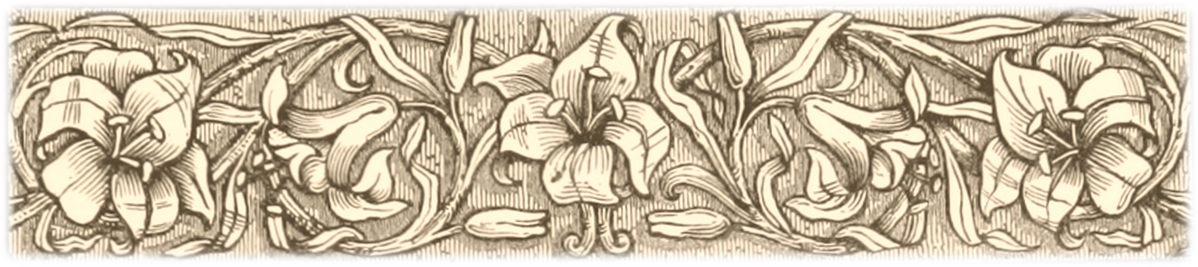
\includegraphics[width=0.9\linewidth]{offene_lizenz/riverdee.png}
\end{center}

\info{
Es empfiehlt sich, im Falle einer sehr kampfschwachen Gruppe die Anzahl der Räuber zu reduzieren oder die Anzahl ihrer schon erlittenen Wunden heraufzusetzen.
}

Sollten die Räuber die Charaktere haben hören können, so haben sie ihre Waffen in der Hand (Holzspeer oder Knüppel), \textbf{Grimma} zielt kniend mit ihrem Kurzbogen auf sie.

\vfill

\zeichnung[0.5\textwidth]{eddard.png}

\kreaturraeuber

Sie werden nicht bis zum Tode kämpfen und sind bei fünf Einschränkungen \textit{kampfunfähig} (also keine Probe auf Zähigkeit, um handlungsfähig zu bleiben). Sobald die Mehrheit von ihnen \textit{kampfunfähig} ist, wird der Rest sich ergeben. Sie lassen sich widerstandslos fesseln und geben zu, dass sie vor ein paar Tagen dem Grafen nur knapp entkommen sind, weshalb sie auch nur wenig Hab und Gut bei sich tragen.
Die Charaktere müssen sich allerdings jetzt entscheiden, was sie mit den Gefangenen machen. Sie hier festzubinden, um sie später abzuholen, ist natürlich machbar.

Sollten die Charaktere unterliegen, werden die Räuber ihnen alles abnehmen, was sie am Leibe tragen und gefesselt zurücklassen. 

\info{
In diesem Fall sieht der Autor nur eine Lösung des Dilemmas: \textbf{Janne} und \textbf{Vittel} haben mittlerweile das Ansinnen des Einhorns verstehen und die Phiole vernichten können. Jetzt befinden sie sich auf dem Rückweg nach Wengenholm und können den Charakteren zu Hilfe eilen. Eine zusätzliche Belohnung haben diese sich zwar nicht verdienen können, 15 EP für ihre Mühen sind allerdings möglich.
}

Sollten die Charaktere die Räuber nicht schon auf dem Weg gehört haben, so konnten die Räuber sie bemerken, sofern sie beim Betreten des Waldes sich nicht bewusst für's Schleichen entschieden hatten. Die Bande wird dann vorauseilen und den Charakteren auflauern. Dabei kniet sich \textbf{Grimma} hinter einen Baumstamm und schießt mit ihrem Bogen aus etwa zehn Schritt Entfernung auf den am stärksten aussehenden Helden, während die anderen aus etwa acht Schritt Entfernung auf die Charaktere zustürmen. 


\mprobe{wahrnehmung}{Wachsamkeit (I, 8+X)}{Wahrnehmung}{
Die Charaktere gelten als \textit{überrascht}, sofern ihnen vorher keine vergleichende Probe gegen -- aufgrund der gut gewählten Deckung höherem -- Pirschen
der Räuber gelingt.
}

\info{
Die Räuber sind bei fünf Einschränkungen \textit{kampfunfähig} und geben auf, sobald einer von ihnen \textit{kampfunfähig} wird.\\Unterliegen die Helden, nehmen die Räuber ihnen alles ab und lassen sie gefesselt zurück.
}


\abschnitt{Jannes Heim}

Sind die Charaktere aus dem Kampf siegreich ausgegangen und haben die gefangen genommenen Räuber gut verschnürt, so gelangen sie ohne weiteres nach etwa einer weiteren Stunde auf eine kleine Lichtung an einem südlich ausgerichteten, schwach absteigenden Hang. Ein kleines Fachwerkhaus auf steinernen, kniehohen Fundamenten blickt über einen größeren Garten. Die Eingangstür an der östlichen Stirnfront des Hauses allerdings steht sperrangelweit offen.


Die Charaktere können das Haus betreten oder zunächst die Umgebung erkunden, in beiden Fällen können sie herausfinden, dass die Hintertür vom Garten aus mit Gewalt eingerannt wurde.

\mprobe{wahrnehmung}{Sinnenschärfe (12)}{Wahrnehmung}{
Ein Pferd muss die Hintertür eingerannt haben und in das Haus gestürmt sein. 
}


Die Küche nebenan ist teilweise verwüstet, und zwar lediglich im direkt an die Hintertür angrenzenden Bereich. Außerdem wurde ein Tisch mit allerlei Kräutern und Gewürzen umgeworfen, der neben der Tür zum Flur gestanden hatte und jetzt vor der Tür liegt. Er lässt sich ohne weiteres von beiden Seiten übersteigen.
\mprobe{wahrnehmung}{Sinnenschärfe (12)}{Wahrnehmung}{
Zwei Personen sind von der Küche aus in das Haus geflohen. 
}


Ist der Erfolgswert der Probe 16 oder höher, so lässt sich sogar feststellen, dass die Fliehenden den Tisch hinter sich umgekippt haben und auf direktem Weg aus der Haustür ins Freie hinaus geflohen sein müssen. 


Die weiteren Räume des Hauses sind eine Stube sowie ein Schlafzimmer. Alles ist einfach, aber bequem ausgestattet. In der Stube befindet sich neben ein paar Sitzgelegenhei-ten um einen niedrigen Tisch eine verschlossene Bücherkiste. Das lässt sich mit einem flüchtigen Blick in die Zimmer feststellen. Die Bücherkiste enthält neben einigen humorvoll geschriebenen Kaiser-Valpo-Geschichten ein Kompendium über die Heil- und Nutzpflanzen des nördlichen Koschs sowie verschiedene Abhandlungen zur Anwendung von \textbf{Magica Contraria} (Antimagie) der \textbf{Akademie der Magischen Rüstung zu Gareth}.

Sollten die Charaktere die Umgebung vor dem Eingangsbereich des Hauses untersuchen, können sie eine weitere Probe ablegen:

\mprobe{wahrnehmung}{Sinnenschärfe (12)}{Wahrnehmung}{
Zwei Personen müssen auf diesem Weg das Haus verlassen haben. 
}
Ist der Erfolgswert der Probe 16 oder höher, so lässt sich sogar feststellen, dass die beiden beim Verlassen gerannt sind, und zwar vor nicht allzu langer Zeit.

Die Spuren lassen sich ohne Probleme bis zum Waldrand verfolgen. Dort können die Charaktere Hilferufe vernehmen, denen sie relativ leicht folgen können.
\begin{center}
\zeichnung[0.5\textwidth]{alchemie.jpg}	
\end{center}

\neuespalte

\abschnitt{Am Ziel}
Auf einem Baum in etwa fünf Schritt Höhe können sie \textbf{Janne Pflögler} und \textbf{Vittel} erkennen.
	Beide befinden sich ganz offensichtlich nicht in bester Verfassung, die Kleidung ramponiert, Schrammen an Händen und Gesicht.
	Zu Füßen des Baumes scharrt ein schneeweißes \textbf{Einhorn} mit den Hufen und schnaubt in Richtung der beiden.
	
	\textbf{Vittel} ruft den Charakteren sofort zu, sobald er sie sieht.
	In dem Augenblick aber wird das \textbf{Einhorn} sich umwenden, einige Schritt auf die Charaktere zulaufen (bis es etwa zehn Schritt vom Baum entfernt ist) und sie mit seinen Gedankenbildern bedrängen.
	Diese sind im Gegensatz zu Drachen keine Gedankensprache, da Einhörnern die Fähigkeit zur Abstraktion ihrer Geisteswelt fehlt.
 

\probenkasten[
    bild=wahrnehmung,
    gruppenprobe=nein,
    zusammenarbeit=nein,
    farbe=blau,
    pw=24,
    anzahl=1,
]
{Magieresistenz}{Ähnlich dem Zauber \biglittlecap{Gedankenbilder Elfenruf} können jedoch alle Charaktere versuchen, das Empfangen der Bilder mit einer \textit{Konterprobe} zu verhindern.}

Alle Charaktere, denen die \textit{Konterprobe} misslingt, werden  regelrecht überwältigt von Bildern eines grausam verendenden Tieres, dem das Alicorn aus der Stirn geschnitten wurde sowie verzerrten Bildern von Menschen, die das Alicorn zu feinem Staub mahlen. Jeder betroffene Charakter muss eine Probe auf Willenskraft ablegen


\mprobe{selbstbeherrschung}{Willenskraft (I, 16)}{Selbstbeherrschung}{
Ein Misslingen macht einige Momente benommen. Dies hat zwar keine direkten Auswirkungen auf den Fortgang des Geschehens, soll den Charakteren aber die arkane Macht des Einhorns vor Augen führen.}

Sollte den Spielenden noch nicht klar geworden sein, dass ein Angriff auf ein Einhorn, dem heiligen Tier des Halbgottes Nandus, für normale Aventurier einen Frevel darstellt, so wäre jetzt der richtige Moment gekommen, es beiläufig zu erwähnen.


Das Zauberwesen wird die Charaktere nicht angreifen, sie allerdings auch nicht auf weniger als zwölf Schritt an den Baum heranlassen.
Da es ständig laut schnaubt, ist eine fehlerlose Verständigung mit \textbf{Vittel} und \textbf{Janne Pflögler} nicht möglich.
\textbf{Janne} hatte nach den ersten Gedankenbildern des \textbf{Einhorn}s sich mit Antimagie versucht zu schützen.
Dafür hatte sie zunächst den Zauber \biglittlecap{Verständigung stören} mit der Modifikation \textit{Zauber aufheben} gewirkt, noch bevor das \textbf{Einhorn} versuchen konnte, ihr vom zermahlenen Alicorn zu berichten.
Während das \textbf{Einhorn} noch verblüfft war, dass die junge Hexe versuchte, sich gegen seine Kontaktaufnahme zu wehren, wirkte \textbf{Janne} den Zauber \biglittlecap{Verständigung stören} mit der Modifikation \textit{Magie unterdrücken}.
Allerdings muss sie den Zauber stündlich neu wirken, um nicht von den Bildern des \textbf{Einhorn}s überwältigt zu werden.
Dadurch besitzt sie noch gerade genug Astralenergie, um ein kleines Ästchen mit einer kurzen, geschriebenen Nachricht per \biglittlecap{Hexenholz} den Charakteren zunächst zukommen und wieder zurückfliegen zu lassen. 


\textbf{Janne} befindet sich unter Schock und schafft es daher nicht, die Botschaften des \textbf{Einhorn}s zu verstehen.
Die Charaktere müssen also versuchen, den Bedrängten klarzumachen, dass das \textbf{Einhorn} bei ihnen zerriebenes Alicorn eines gewaltsam getöteten Einhorns vermutet.
Das \textbf{Einhorn} wird die Charaktere nicht an den Baum heranlassen, ein Überklettern von benachbarten Bäumen ist dagegen möglich.
Letztlich sollte jede halbwegs logische Idee von Seiten der Spielenden honoriert werden.


Sobald \textbf{Vittel} die tatsächliche Absicht des \textbf{Einhorn}s verstanden hat, wird er die Phiole auf den Boden werfen, wo sie vom \textbf{Einhorn} sofort zertreten und der Inhalt mit den Hufen in den Waldboden gestampft wird.
Anschließend verschwindet die magische Kreatur mit einem letzten Schnauben genauso schnell im Wald, wie sie erschienen ist.


\textbf{Vittel} und \textbf{Janne} sollten dann vom Baum klettern können, abgesehen von ein paar Kratzern körperlich wohlbehalten, die Knie noch schlotternd vom Schreck.
\textbf{Janne} setzt sich erst einmal auf den Waldboden, um ihre Gedanken zu sammeln. Schnell kann sie wieder klar denken und begreift das Geschehene. Im Zweifelsfall kann sie die Charaktere über den Hintergrund der Phiole aufklären.

Sowohl \textbf{Vittel} als auch \textbf{Janne} werden sich sehr dankbar zeigen, die junge Hexe sie in die Stube ihres Hauses einladen und erst einmal einen kräftigenden Tee aufbrühen, zu dem sie noch leckere Haferplätzchen stellt.
Zum Dank gibt sie den Charakteren eine Feldflasche mit 3 Portionen Einbeerentrank (1\,x\,HQ), der noch 18 Monde haltbar ist, ein Döschen mit 2 Erschöpfungspastillen, die noch 12 Monde haltbar sind sowie ein Tiegelchen mit 2 Portionen Brandsalbe (2\,x\,HQ).
\textbf{Vittel} bezahlt sie einen anständigen Preis für den Heiltrank (den sie nicht bereit ist, weiter zu veräußern, geschweige denn zu verschenken).


Anschließend begleitet sie \textbf{Vittel} und die Charaktere bis \textbf{Wengenholm}.
Sollten sich am Rande des Weges im Wald noch gut verschnürte Räuber befinden, so kann \textbf{Janne} bei der Ablieferung in der Angenburg behilflich sein.
Der \textbf{Burgvogt} wird den Charakteren außer den 5 Dukaten Kopfgeld pro Räuber eine warme Mahlzeit sowie ein Dach über dem Kopf für die anbrechende Nacht anbieten.
\textbf{Vittel} wird bei \textbf{Janne} in der gräflichen Schreibstube übernachten, so dass die beiden sich jetzt verabschieden und das Abenteuer zu seinem Ende kommt. 

\abschnitt{Der Mühen Lohn}
Neben den Alchimika und den hoffentlich durch die Ergreifung der Räuber verdienten Dukaten gibt es auch noch \textit{30 EP} für die durchgemachten Strapazen.

\neuespalte

\abschnitt{Anhang: Dramatis Personae}

\subsection[Vittel, Gehilfe im Peraine-Tempel]{Vittel, Gehilfe im Peraine-Tempel zu Wengerode}
Der sympathische Gehilfe des \textbf{Peraine}-Tempels zu \textbf{Boggerode} entspricht mit seinem vollen, schwarzen Haaren und dem dichten Vollbart ganz dem Bild des typischen Koschers.
Trotz seiner Körpergröße von neuneinhalb Spann ist der 21-jährige recht behändig.
Er kann nicht nur Lesen und Schreiben, sondern ist auch sehr erfahren im Umgang mit Pflanzen und Tieren.
Nicht nur mit seinem Bartwuchs, auch mit seiner Liebe für das Hopfenbräu ähnelt er den Angroschim.


\absatz{Janne Pflögler, gräfliche Schreiberin}
Die gutaussehende Hexe mit dem langen rotbraunen Haar ist nicht nur als Schreiberin für Graf \textbf{Jallik} tätig, sondern steht ihm bei wichtigen Anlässen auch als diskrete Beraterin arkanen Fragen und sogar als magische Beschützerin zur Seite. Allerdings führt ihre schnelle Reaktionsfähigkeit dazu, dass sie die Gedankensprache des \textbf{Einhorn}s als magischen Angriff wahrnimmt und sofort mit Antimagie unterbricht.

Sie kleidet sich praktisch mit einer einfachen, hellen Leinenbluse und einer weiten, dunkelbraunen Hose, in deren Taschen sich ihre Smaragdnatter \textbf{Havel} versteckt hält. Ihr Beruf lässt sich an ihren stets mit Tinte befleckten Händen leicht erkennen.

\spaltenende